\documentclass[12pt,a4paper]{article}
\usepackage[utf8]{inputenc}
\usepackage[T2A]{fontenc}
\usepackage[english,russian]{babel}
\usepackage[a4paper, mag=1000, left=1.5cm, right=2cm, top=2cm, bottom=2cm, headsep=0.7cm, footskip=1cm]{geometry}
\usepackage{amsmath}
\usepackage{pgfplots, colortbl}
\usepackage{makecell}
\usepackage{multicol}
\usepackage{pgfplotstable}
\pgfplotsset{compat=1.16}
\usepackage{minted}
\usepackage{listings}
\usepackage{lstfiracode}
\usepackage{mathrsfs}
\usepackage{graphicx}
\usepackage{caption}
\usepackage{subcaption}

\usemintedstyle{colorful}
\newenvironment{code}{\captionsetup{type=listing}}{}


\newcommand{\smalltable}[1]{
	\pgfplotstabletypeset[
	string type,
	col sep=comma,
	columns/name/.style={column name=Метод, column type={|c}},
	columns/x1/.style={column name=$x_1$, column type={|c}},
	columns/x2/.style={column name=$x_2$, column type={|c}},
	columns/num/.style={column name=Количество итераций, column type={|c|}},
	every head row/.style={before row=\hline, after row=\hline},
	every last row/.style={after row=\hline}
	]{#1}
}

\newcommand{\funtable}[1]{
	\pgfplotstabletypeset[
	every even row/.style=
	{before row={\rowcolor[gray]{0.95}}},
	string type,
	columns/number/.style={column name=№, column type={|c}},
	columns/x1/.style={column name=$x_1$, column type={|c}},
	columns/x2/.style={column name=$x_2$, column type={|c}},
	columns/x3/.style={column name=$x_3$, column type={|c}},
	columns/x3/.style={column name=$x_3$, column type={|c}},
	columns/alpha/.style={column name=$\alpha$, column type={|c}},
	columns/steps/.style={column name=\makecell[b]{Итераций \\одномерного\\поиска}, column type={|c|}},
	every head row/.style={before row=\hline, after row=\hline},
	every last row/.style={after row=\hline}
	]{data/methods/#1.csv}
}

\newcommand{\imgs}[1]{
	
	\hbox to\linewidth{
		\vbox{
			\hbox{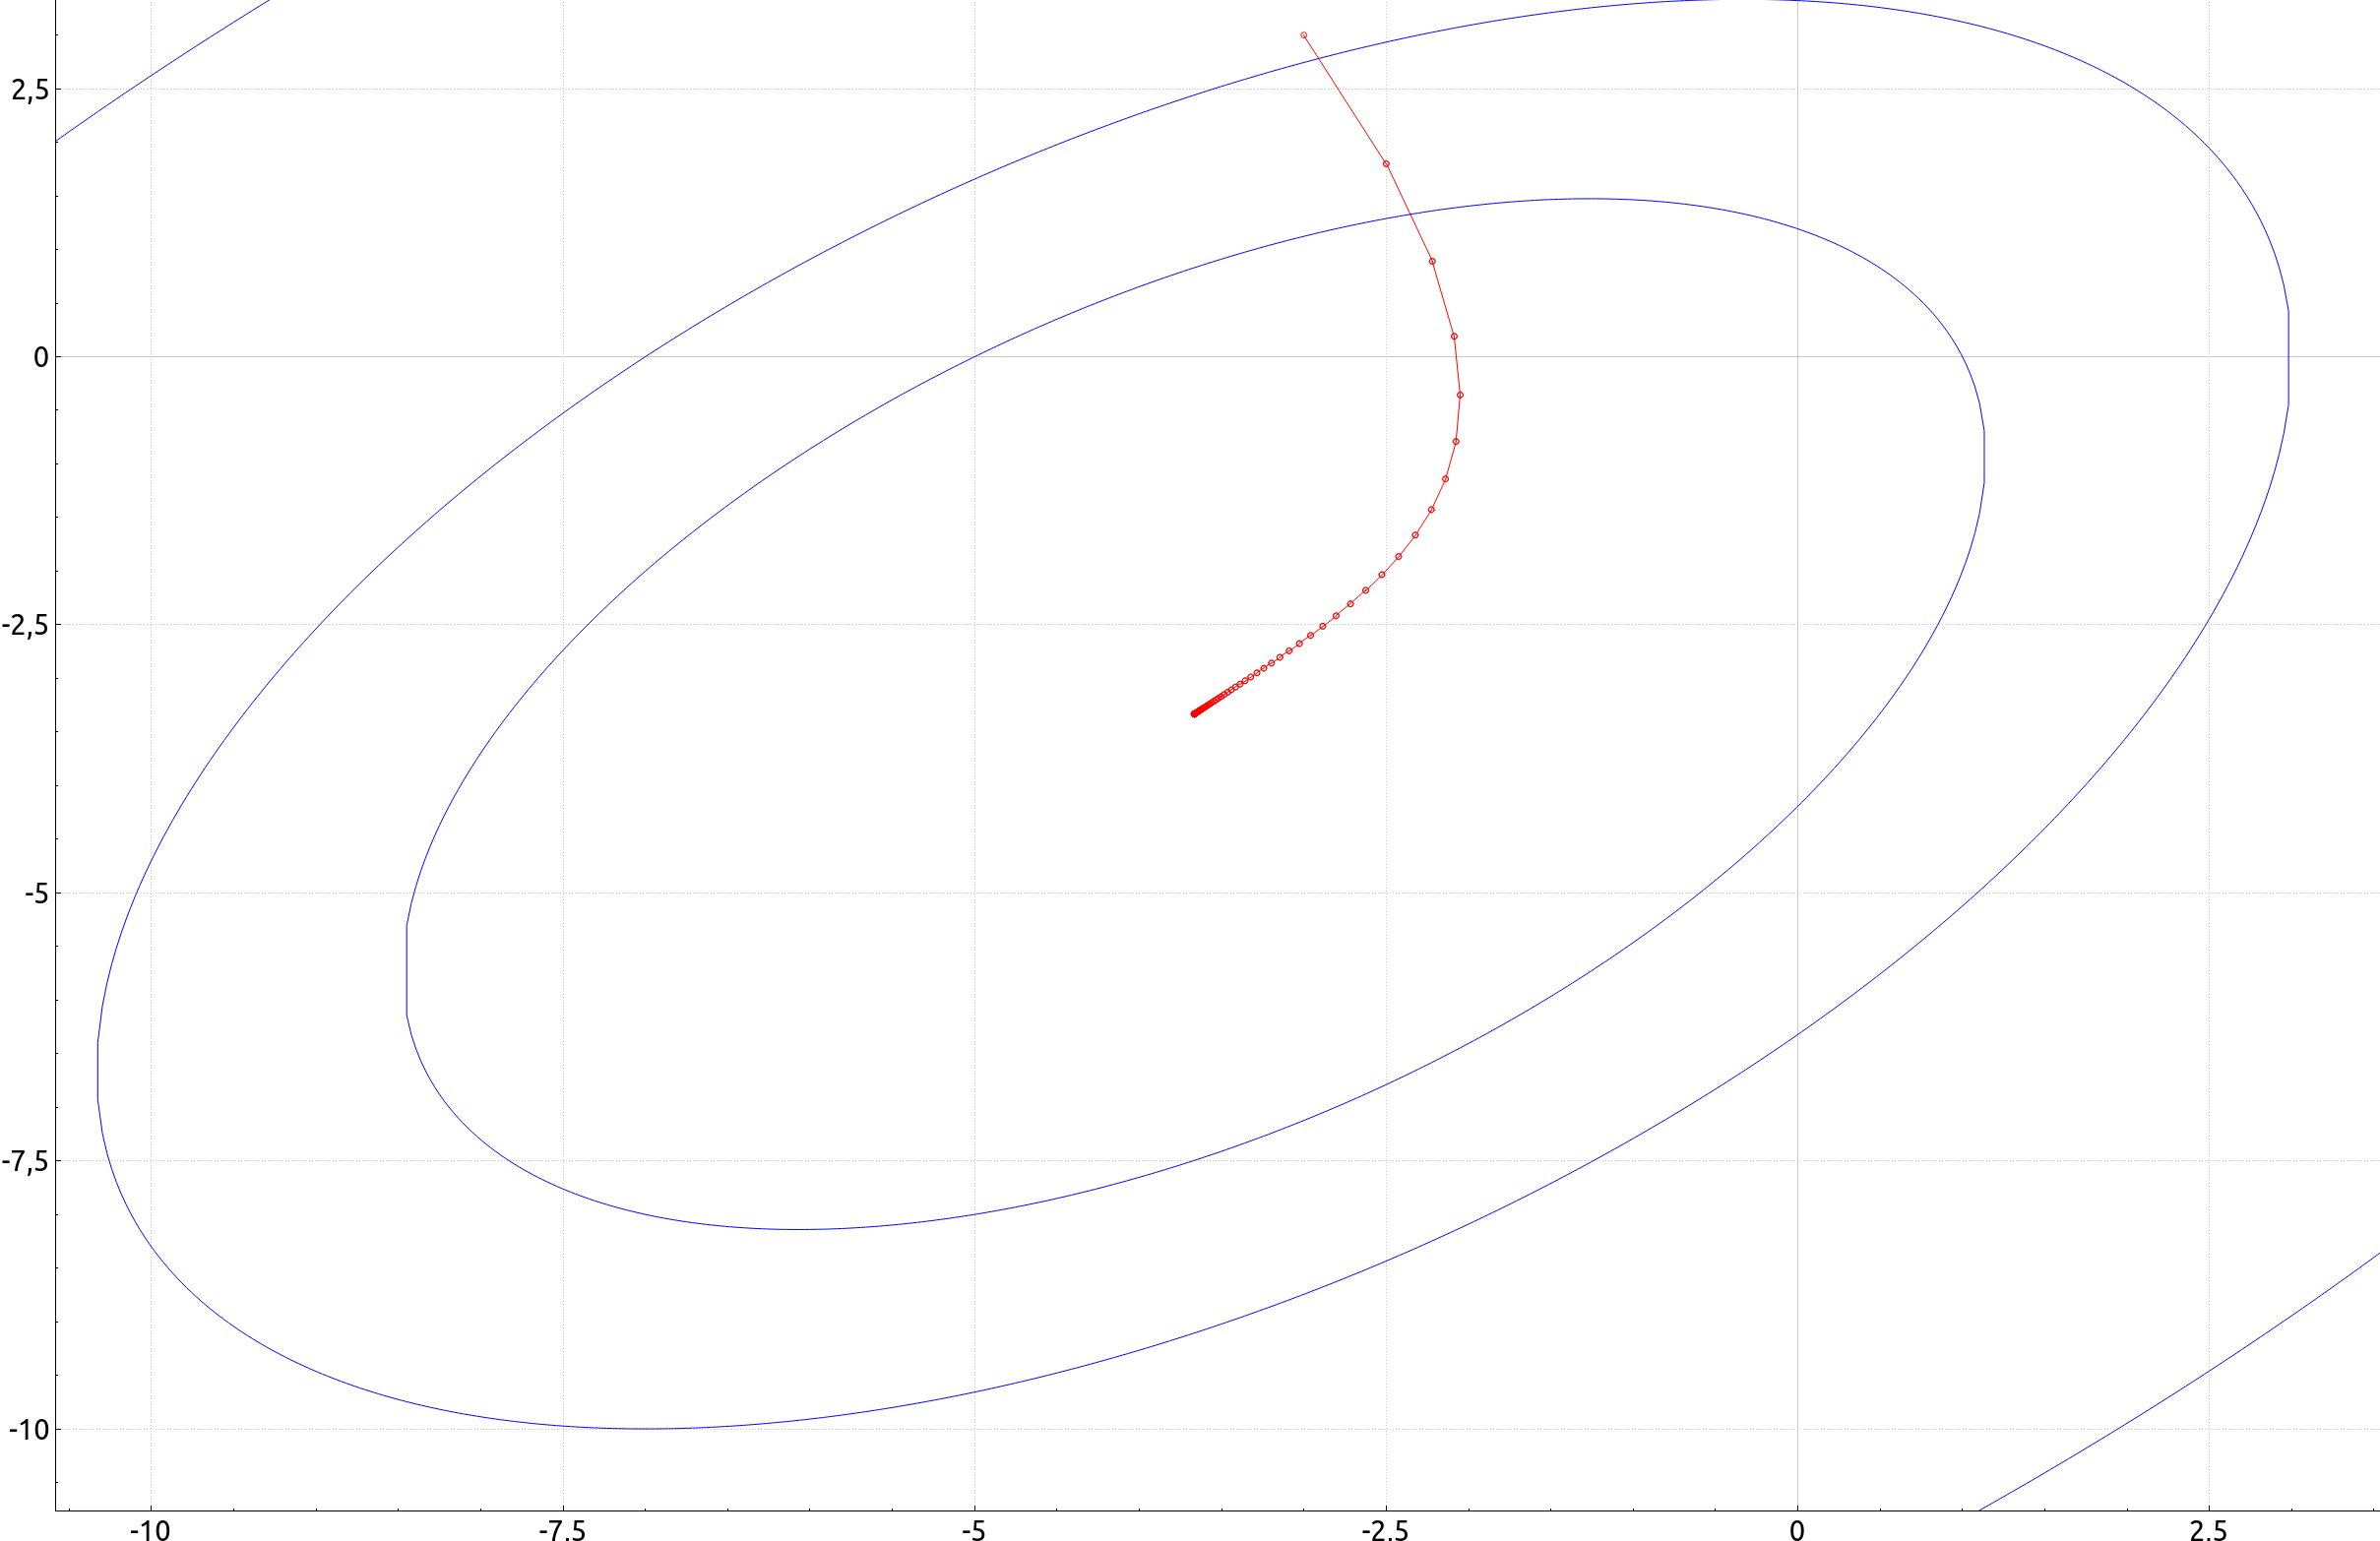
\includegraphics[width=.5\textwidth,
				height=.4\textwidth]{img/#1/g.jpg}}
			\hbox{Градиентный спуск}
		}
		\t
		\hfill
		\vbox{
			\hbox{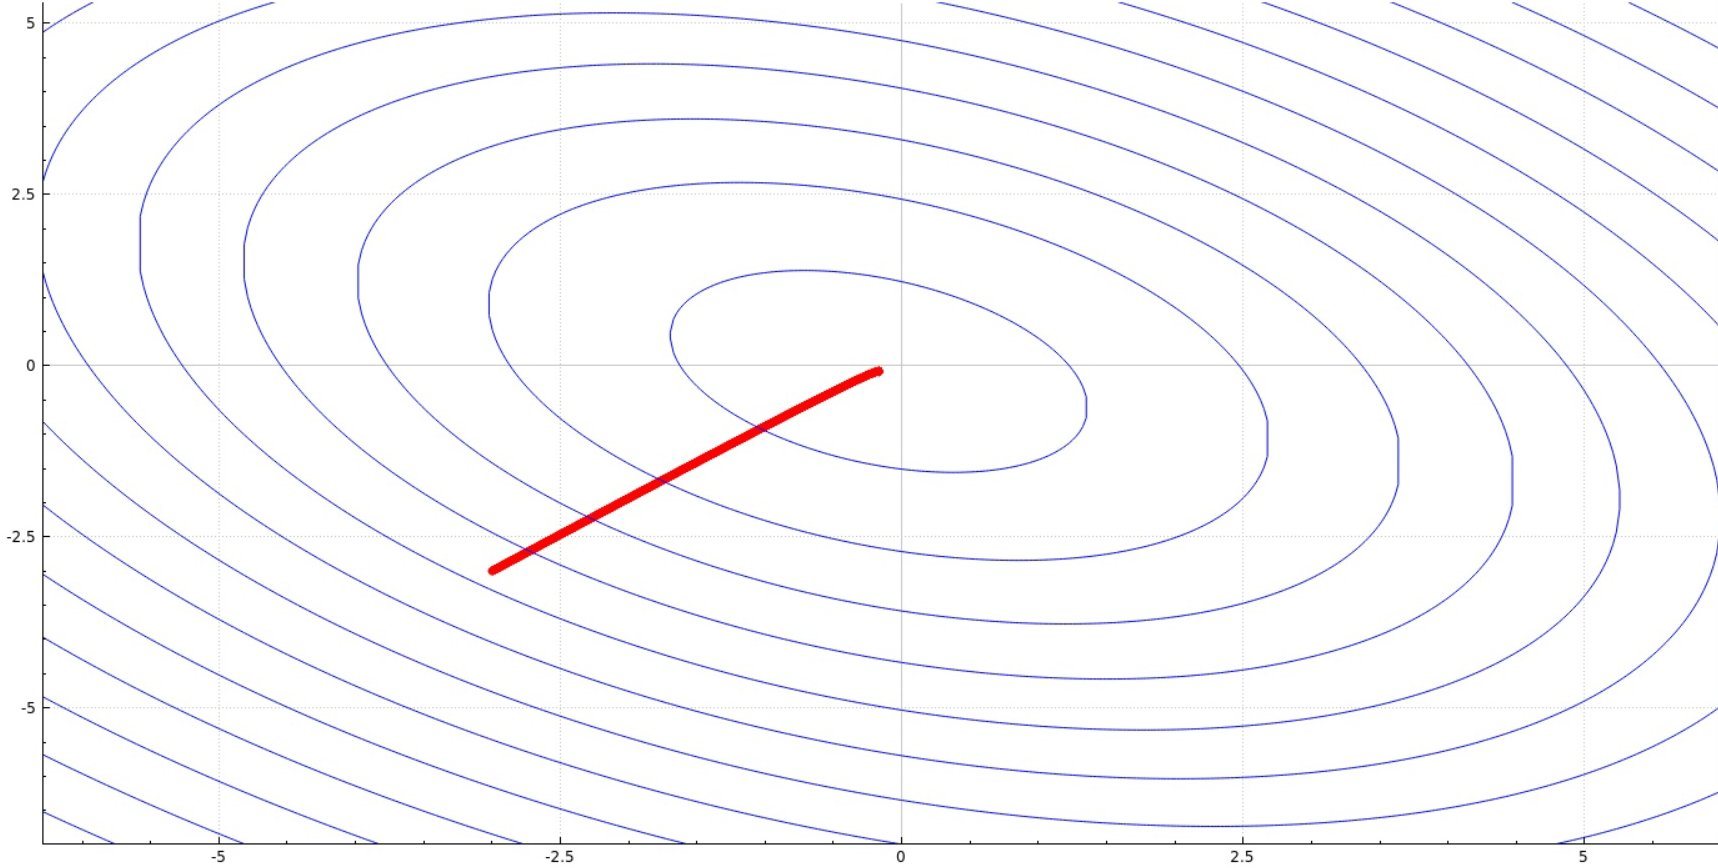
\includegraphics[width=.5\textwidth,
				height=.4\textwidth]{img/#1/f.jpg}}
			\hbox{Наискорейший спуск}
		}
	}

	
	\vbox{
		\hbox{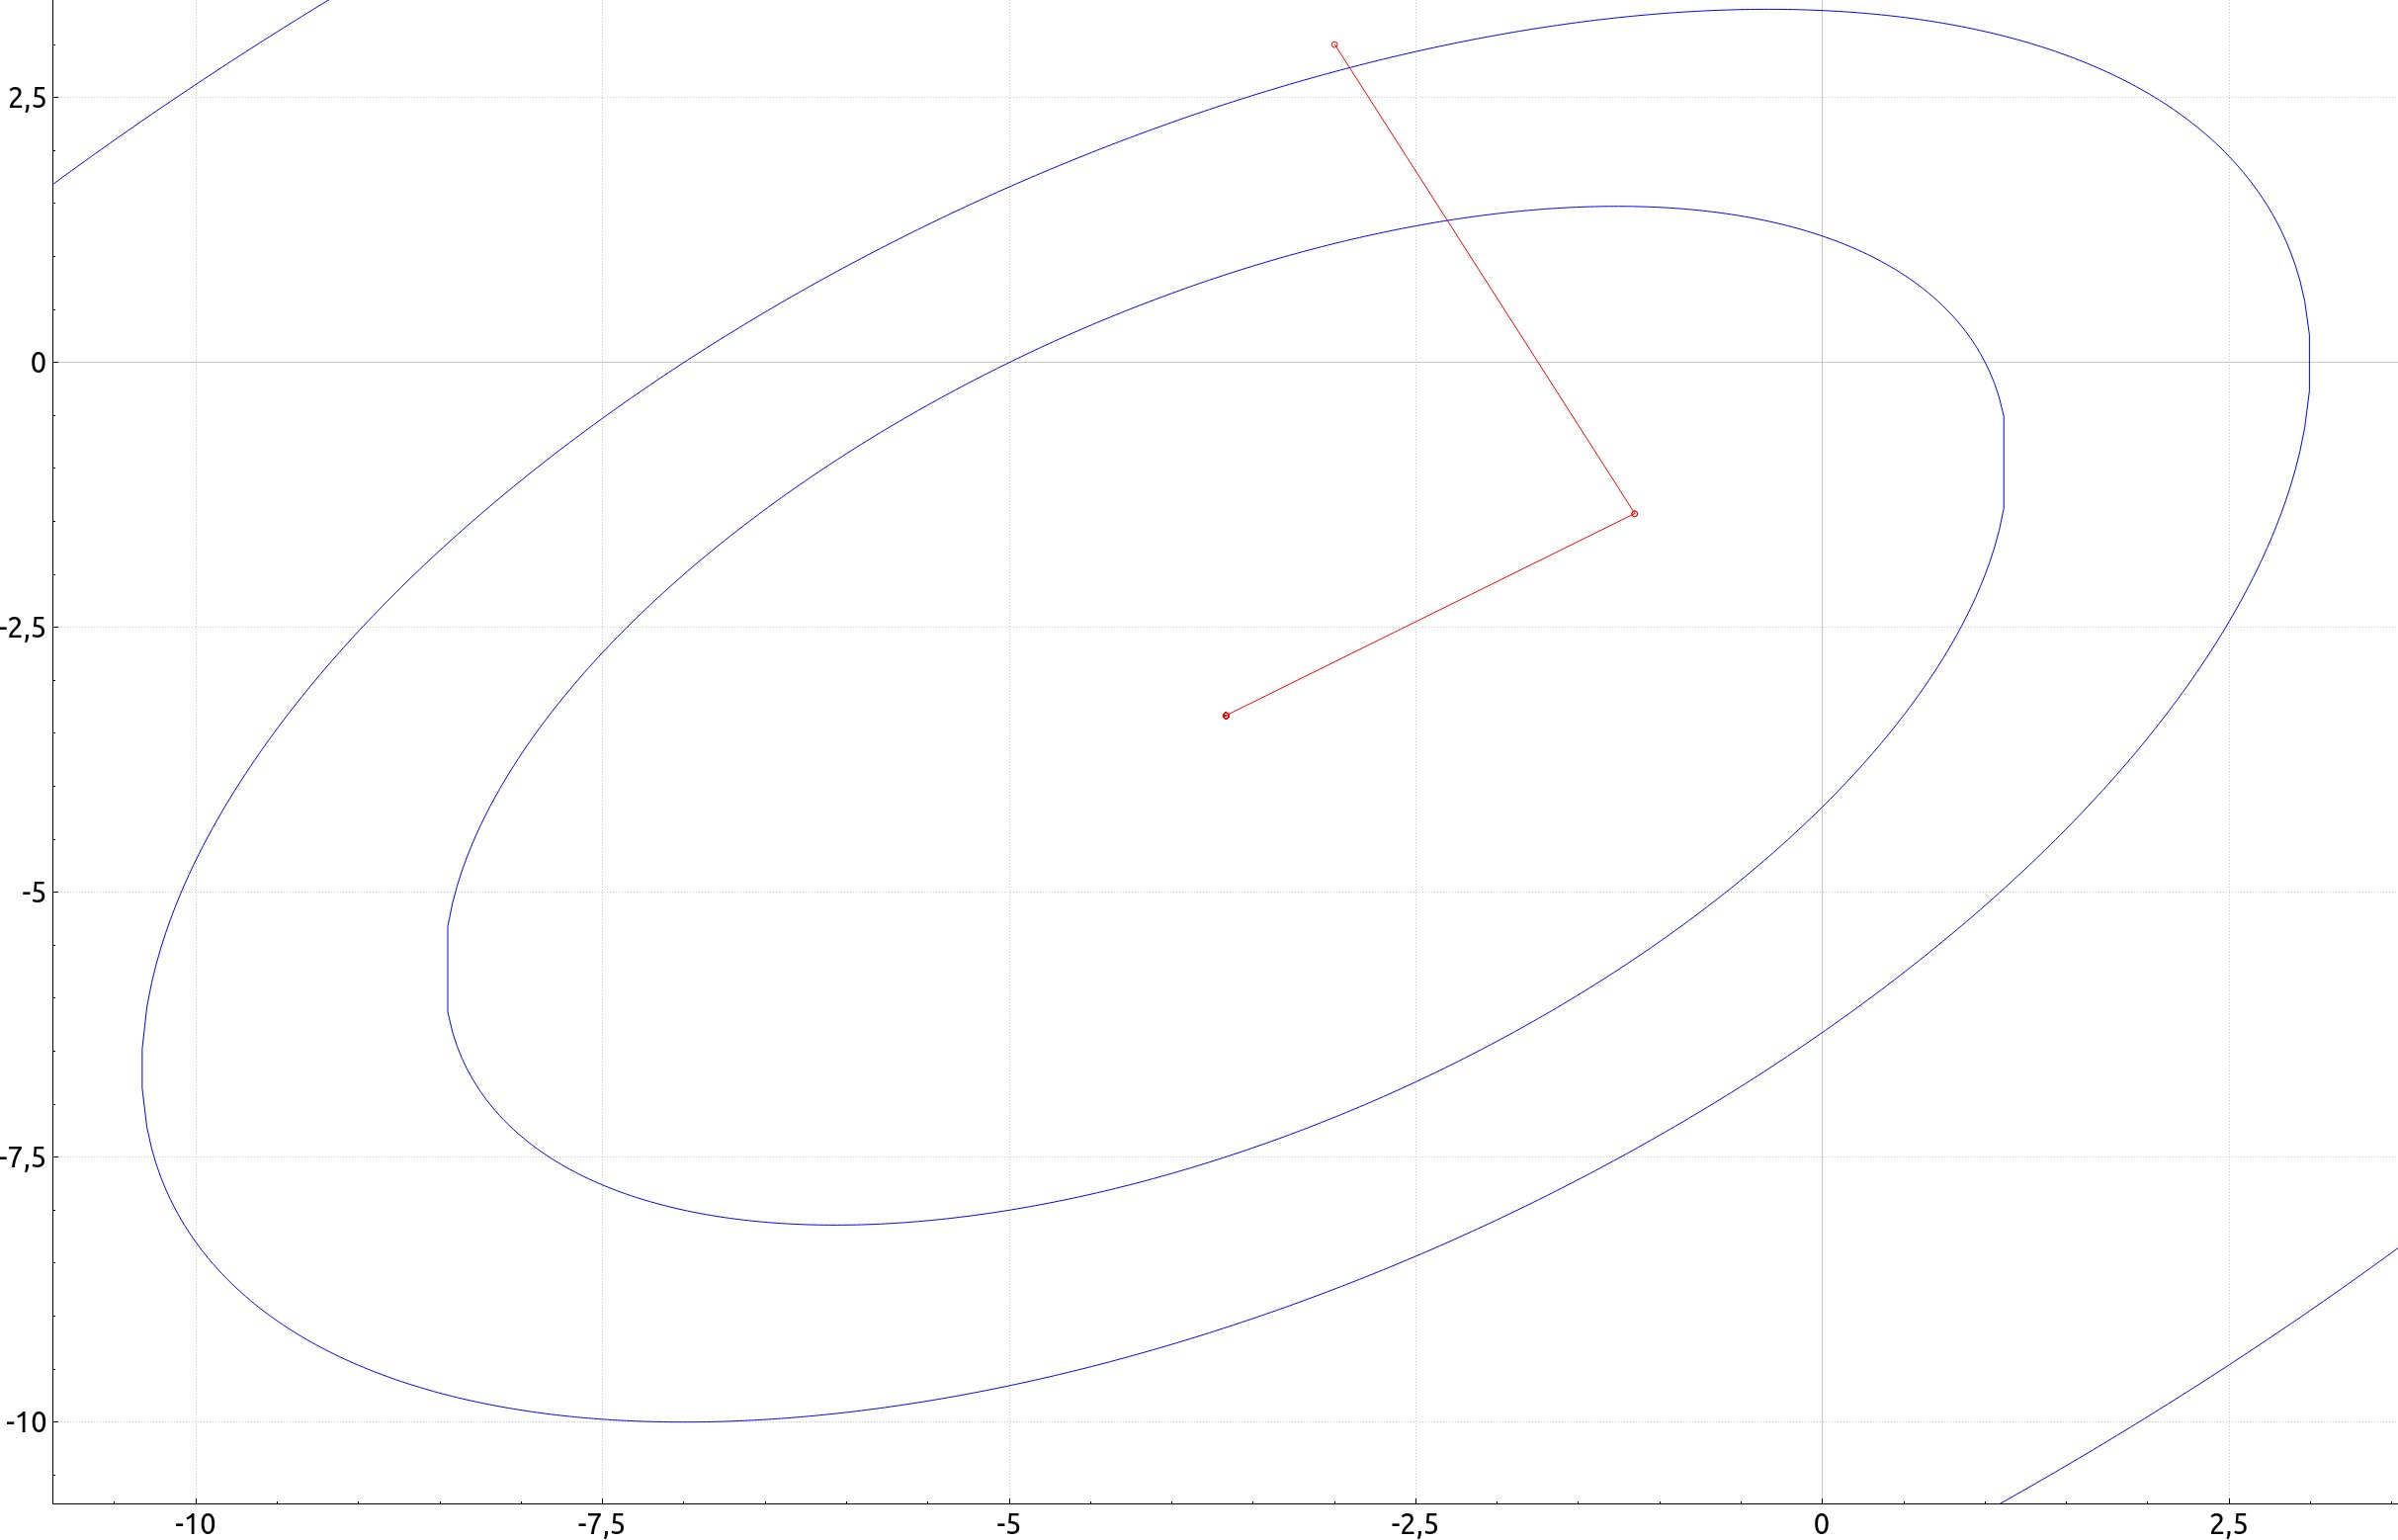
\includegraphics[width=.5\textwidth,
			height=.4\textwidth]{img/#1/c.jpg}}
		\hbox{Сопряженные градиенты}
	}

}

\newcommand{\kngraph}[1] {
	\begin{center}
		\begin{tikzpicture}
		\begin{semilogxaxis}[
		title = {},
		xlabel = $k$,
		ylabel = number of iterations,
		legend pos=outer north east,
		width=0.8\textwidth,
		]
		\addplot table [x={k}, y={number}] {data/#1/n1.csv};
		\addplot table [x={k}, y={number}] {data/#1/n2.csv};
		\addplot table [x={k}, y={number}] {data/#1/n3.csv};
		\addplot table [x={k}, y={number}] {data/#1/n4.csv};
		\addlegendentry{$n = 10$}
		\addlegendentry{$n = 10^2$}
		\addlegendentry{$n = 10^3$}
		\addlegendentry{$n = 10^4$}
		\end{semilogxaxis}
		\end{tikzpicture}
	\end{center}
}

\newcommand{\mcode}[1]{
    \begin{code}
        %\caption*{#1}
        \inputminted[breaklines=true, xleftmargin=1em, linenos, frame=single, framesep=10pt, fontsize=\footnotesize]{cpp}{#1}
    \end{code}
}